\documentclass[12pt]{article}
\usepackage[margin=1in]{geometry}
\usepackage{amsmath}
\usepackage{amssymb}
\usepackage{graphicx}
\usepackage{caption}
\usepackage[colorlinks=true,urlcolor=red]{hyperref}
\usepackage{color}
\usepackage{enumerate}

\begin{document}
\title{Firewall Intermediate Report}
\author{Akshay Dongaonkar (akd54)}
\maketitle

\section{Objective}

I will be implementing a firewall on a Linux-based kernel that mediates
access to an internal network. 
Given time, I will also implement a DMZ where components of the network
may live outside the firewall if they need to.
This project will be developed incrementally. 
I will first implement a stateless firewall.
This means that every packet will be analyzed. 
I will then test the scalability of such an approach and
implement a stateful approach.
The implementation of the stateful approach will be discussed in the code
section.

\section{Firewall Language Grammar}

The firewall language grammer is what tells our program which packets to block
and which packets to allow through to our internal network.
We need this grammar so our program parses packets correctly.
The firewall language grammar will be implemented incrementally.
I will primarily leverage the pcap-filer functionality to implement many of
these rules.
The rule syntax will generally follow the BSD syntax used in HW2.
That syntax is as follows. \par
\begin{verbatim}
action [direction] [log] [quick] [on interface] [af] [proto protocol] \
   [from src_addr [port src_port]] [to dst_addr [port dst_port]] \
   [flags tcp_flags] [state]
\end{verbatim}

We will not be implementing the log facility right now.
This will be an extension at the end of the project cycle, because
there needs to be a way to move the logged file from the firewall to the
device that requested the shot.
The easiest way to accomplish that is to create a HTTP server that interacts
with users within the network.
The second easiest way to implement the log facility is to name the log file
and store it in a well known location.
A user within the network can then FTP the file over with the well known
details.  \par

In the same vein, the interface of capture will be the single input 
interface to our firewall.
This is dependent on the environment the firewall is running on,
but generally there is one interface from which we are mediating access.
If we want to mediate internal traffic, we will of course need to 
accept from multiple interfaces. 
This will be implemented after we implement logging.

The rest of the fields can be translated generally one-to-one to pcap
filtering rules.

\section{Code and Data Structures}

Right now, there is a simple loop and a simple handler that grab packets off
of the currently used interface. 
The handler for the packets captured linearly checks against a filter string.
This is not extensible as there is only one rule in effect at all times. \par

The reason this happened was that I was basing a lot of my code from the
libpcap tutorial provided by
\href{http://yuba.stanford.edu/~casado/pcap/section3.html}{Stanford}.
I will be switching to a different architecture once I resolve an issue
discussed in section 5. \par

The current architecture I have in mind is to have multithreaded pcap capture
loops that grab packets that conform to their firewall rule.
The $n+1^{th}$ rule will specifically avoid packets captured by the $n$ rule
by careful use of the pcap filter expression. 
So, to make things easier for us, our firewall tries to match to the first 
rule, going top to bottom. \par

For a block rule, the captured packet references a special pcap handler that
simply does nothing to the packet.
For a pass rule, we reference a handler that injects the packet to our internal
network interface port.
This will give us most of the functionality that we need for our firewall.
For our DMZ, we have its rules at the top of our rule set.
We then have our capture loop reference a handler that forwards the packet
to the DMZ interface port. \par

However, this will not really scale.
We need a way to maintain states of connections so we do not have handle packet
analysis at every packet.
For large (elephant) streams, this would be very cumbersome.
I am not completely sure as to how I'm going to implement state with my 
pre-existing code structure. \par

As a first step, I will maintain a hashtable of connections hashed by
the source ip address within our network and the destination ip address
outside our network.
This hashed value will refer to a linked list that maintains all the 
connections between the pair.
I anticipate each linked list to have average size 10.
This is because many multiple connections are primarily caused by HTTP.
Most browsers open 1-10 concurrent connections to a source.
If this not true in practice, I will also hash by source and destination ports.
This can only happen if ports exist within the connection protocol, so
a special port number will be given to protocols that do not have ports. \par

Given this somewhat constant lookup time, each loop handler will lookup
whether a connection exists. 
If it does, we skip our updates and analyses and just forward the packet.
I do not know whether I will need this state, as most of the classification
is being done by our pcap filters in our capture loops.
I need to investigate further.

\section{Testing Strategy}

The testing strategy is as follows. 
I will be using my HP laptop which runs Ubuntu 14.04 LTS.
I will capture packets from my \texttt{wlan0} interface to feed to my firewall.
Of course, to test functionality of the rules, I will capture beforehand and
use libpcap's ability to read from pcap files. 
The \texttt{wlan0} interface will primarily test the scalability of my code.
Once the packets are ingested by the program,
the firewall will analyze the packets and match against rules
as described in the aforementioned section.
My firewall will then output the allowed packet on another interface.
Usually this is described by the command line parameters;
my testing instance will rely on the \texttt{eth0} interface on my laptop. \par

To verify our rules work, I will be using the Wireshark tool.
A picture of a sample Wireshark capture all is shown in Figure 1. \\
\begin{figure}[h]
	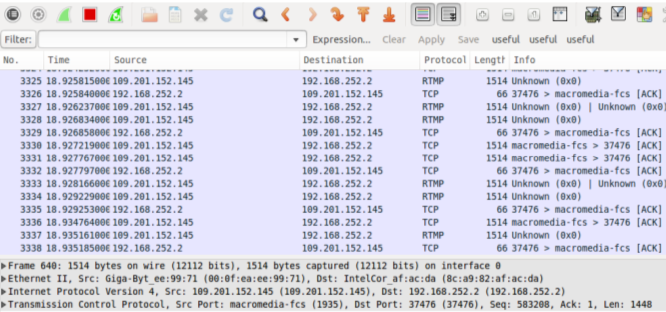
\includegraphics[scale=0.77]{wireshark.png}
	\caption{A sample Wireshark capture on our interface.
			 You can see a streaming TCP connection in the capture.}
\end{figure}
I will capture the \texttt{eth0} interface.
This is very useful as I can see whether my rules accurately work in real time.
I can then replicate my test with a dumped pcap file that Wireshark generates.
The testing then also remains contained to a single machine.
This way, I will not have to deal much with external network rules. \par

Essentially, my firewall becomes a pipe for network packets.
To implement the DMZ and make the firewall more of a switch as it needs to be,
I just need an interface to pipe the DMZ packets.
I then just add rules to pipe packets destined to the DMZ to the appropriate
interface.
That will be one of the last things implemented, as it is a trivial extension
if our system woks. 
It is just reapplying our functionality to implement a new feature.

\section{Progress So Far}

Currently I am able to ingest packets from the \texttt{wlan0} interface and
analyze them with a generic handler.
I am able to implement very simple rules that can be captured via the pcap
filter.
However, I can only implement one rule at a time.
Of course, the block all rule works trivially. \par

The only problem I have with my code right now is exporting out to the
\texttt{eth0} interface.
I anticipate this problem will be solved within the weekend,
as pcap was designed to handle exactly what I am trying to accomplish.


\end{document}